\documentclass{beamer}
\usepackage{amsmath}
\usepackage{hyperref}
\usepackage{listings}
\usepackage{xcolor}
\hypersetup{colorlinks=true, citecolor=blue, filecolor=blue, linkcolor=blue, urlcolor=blue}
\definecolor{codegreen}{rgb}{0,0.6,0}
\definecolor{codegray}{rgb}{0.5,0.5,0.5}
\definecolor{codepurple}{rgb}{0.58,0,0.82}
\definecolor{backcolour}{rgb}{0.95,0.95,0.92}
 
\lstdefinestyle{mystyle}{
    backgroundcolor=\color{backcolour},   
    commentstyle=\color{codegreen},
    keywordstyle=\color{magenta},
    numberstyle=\tiny\color{codegray},
    stringstyle=\color{codepurple},
    basicstyle=\ttfamily\footnotesize,
    breakatwhitespace=false,         
    breaklines=true,                 
    captionpos=b,                    
    keepspaces=true,                 
    %numbers=left,                    
    numbersep=5pt,                  
    showspaces=false,                
    showstringspaces=false,
    showtabs=false,                  
    tabsize=2
}
 
\lstset{style=mystyle}

\mode<presentation> {

% The Beamer class comes with a number of default slide themes
% which change the colors and layouts of slides. Below this is a list
% of all the themes, uncomment each in turn to see what they look like.

%\usetheme{default}
\usetheme{AnnArbor}
%\usetheme{Antibes}
%\usetheme{Bergen}
%\usetheme{Berkeley}
%\usetheme{Berlin}
%\usetheme{Boadilla}
%\usetheme{CambridgeUS}
%\usetheme{Copenhagen}
%\usetheme{Darmstadt}
%\usetheme{Dresden}
%\usetheme{Frankfurt}
%\usetheme{Goettingen}
%\usetheme{Hannover}
%\usetheme{Ilmenau}
%\usetheme{JuanLesPins}
%\usetheme{Luebeck}
%\usetheme{Madrid}
%\usetheme{Malmoe}
%\usetheme{Marburg}
%\usetheme{Montpellier}
%\usetheme{PaloAlto}
%\usetheme{Pittsburgh}
%\usetheme{Rochester}
%\usetheme{Singapore}
%\usetheme{Szeged}
%\usetheme{Warsaw}

% As well as themes, the Beamer class has a number of color themes
% for any slide theme. Uncomment each of these in turn to see how it
% changes the colors of your current slide theme.

%\usecolortheme{albatross}
%\usecolortheme{beaver}
%\usecolortheme{beetle}
%\usecolortheme{crane}
%\usecolortheme{dolphin}
%\usecolortheme{dove}
%\usecolortheme{fly}
%\usecolortheme{lily}
%\usecolortheme{orchid}
%\usecolortheme{rose}
%\usecolortheme{seagull}
%\usecolortheme{seahorse}
%\usecolortheme{whale}
%\usecolortheme{wolverine}

%\setbeamertemplate{footline} % To remove the footer line in all slides uncomment this line
\setbeamertemplate{footline}[page number] % To replace the footer line in all slides with a simple slide count uncomment this line

\setbeamertemplate{navigation symbols}{} % To remove the navigation symbols from the bottom of all slides uncomment this line
}

\usepackage{graphicx} % Allows including images
\usepackage{booktabs} % Allows the use of \toprule, \midrule and \bottomrule in tables
%\usepackage {tikz}
\usepackage{tkz-graph}
\GraphInit[vstyle = Shade]
\tikzset{
  LabelStyle/.style = { rectangle, rounded corners, draw,
                        minimum width = 2em, fill = yellow!50,
                        text = red, font = \bfseries },
  VertexStyle/.append style = { inner sep=5pt,
                                font = \normalsize\bfseries},
  EdgeStyle/.append style = {->, bend left} }
\usetikzlibrary {positioning}
%\usepackage {xcolor}
\definecolor {processblue}{cmyk}{0.96,0,0,0}
%----------------------------------------------------------------------------------------
%	TITLE PAGE
%----------------------------------------------------------------------------------------

\title[Sampling Plans]{Numerical Optimization 13: Sampling Plans} %

\author{Qiang Zhu} % Your name
\institute[University of Nevada Las Vegas] % Your institution as it will appear on the bottom of every slide, may be shorthand to save space
{
University of Nevada Las Vegas\\ % Your institution for the title page
\medskip
}
\date{\today} % Date, can be changed to a custom date

\begin{document}

\begin{frame}
\titlepage % Print the title page as the first slide
\end{frame}

\begin{frame}
\frametitle{Overview} % Table of contents slide, comment this block out to remove it
\tableofcontents % Throughout your presentation, if you choose to use \section{} and \subsection{} commands, these will automatically be printed on this slide as an overview of your presentation
\end{frame}

%----------------------------------------------------------------------------------------
%	PRESENTATION SLIDES
%----------------------------------------------------------------------------------------

%------------------------------------------------

\section{Sampling}
\begin{frame}{Optimization with expensive function evaluations }
For many optimization problems, function evaluations can be quite expensive. 
\begin{itemize}
    \item an aircraft design may require a wind tunnel test
    \item deep learning hyperparameters may require a week of GPU training
    \item $\cdots$
\end{itemize} 
A common approach for optimizing in these contexts is to build a \textcolor{blue}{surrogate model},
Further evaluations of the true objective function can be used to improve the model. Fitting such models requires an initial set of points, ideally points that are space-filling; that is, points that cover the region as well as possible. 
\end{frame}

\section{Full Factorial}
\begin{frame}{Full Factorial}
The full factorial sampling plan places a grid of evenly spaced points over the search space.
\begin{itemize}
    \item a lower/upper-bound vector $a, b$ such that $a_i \leq x_i \leq b_i$
    \item $m_i$ samples in each $x_i$ separated by a distance $(b_i-a_i)/(m_i-1)$
\end{itemize} 
\begin{figure}
\centering
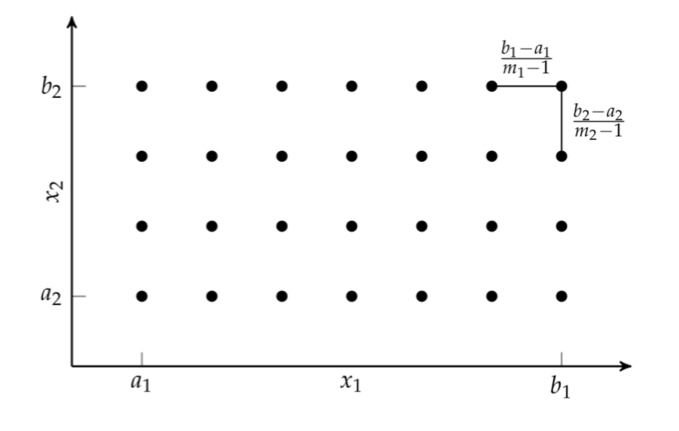
\includegraphics[width=80mm]{Figs/grid_search.jpeg}
\end{figure} 

\end{frame}

\section{Random Sampling}
\begin{frame}{Random Sampling}
In some cases, it may be possible to transform a problem so that constraints can be removed. For example, bound constraints a ≤ x ≤ b can be removed by passing x through a transform

\end{frame}


\section{Uniform Projection Plans}
\begin{frame}{Uniform Projection Plans}
In some cases, it may be possible to transform a problem so that constraints can be removed. For example, bound constraints a ≤ x ≤ b can be removed by passing x through a transform

\end{frame}

\section{Stratified Sampling}
\begin{frame}{Uniform Projection Plans}
In some cases, it may be possible to transform a problem so that constraints can be removed. For example, bound constraints a ≤ x ≤ b can be removed by passing x through a transform


\end{frame}


\section{Space-Filling Metrics}
\begin{frame}{Uniform Projection Plans}
In some cases, it may be possible to transform a problem so that constraints can be removed. For example, bound constraints a ≤ x ≤ b can be removed by passing x through a transform


\end{frame}

\section{Summary}
\begin{frame}{Summary}
    \begin{itemize}
        \item Constraints are requirements on the design points that a solution must satisfy.
        \item Some constraints can be transformed or substituted into the problem to result in an unconstrained optimization problem.
        \item Analytical methods using Lagrange multipliers yield the generalized Lagrangian and the necessary conditions for optimality under constraints.
        \item A constrained optimization problem has a dual problem formulation that is easier to solve and whose solution is a lower bound of the solution to the original problem.
    \end{itemize}
\end{frame}
\end{document}

